


\tikzset{every picture/.style={line width=0.75pt}} %set default line width to 0.75pt        

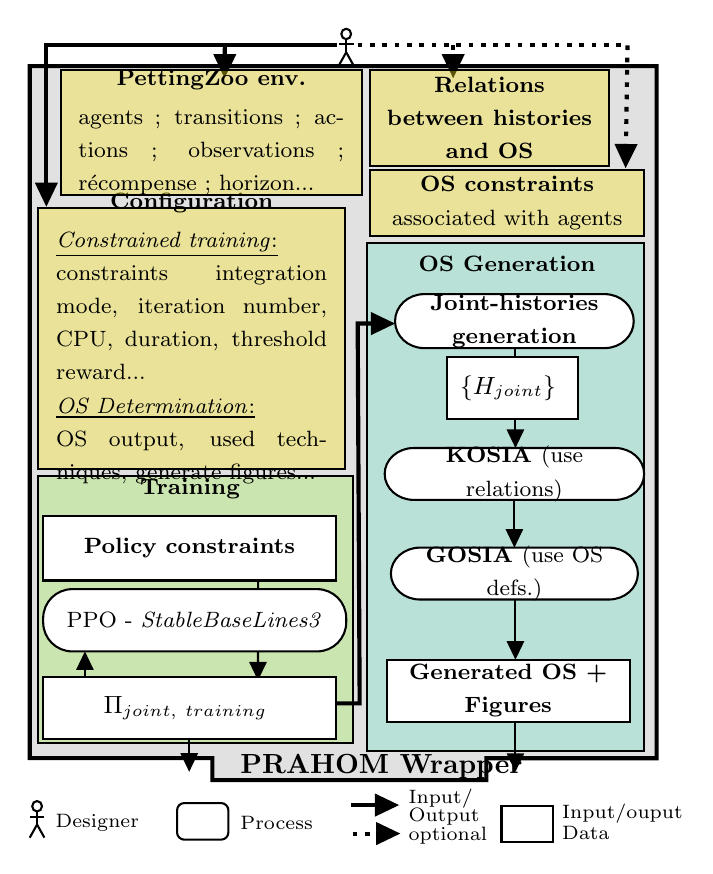
\begin{tikzpicture}[x=0.75pt,y=0.75pt,yscale=-1,xscale=1]
%uncomment if require: \path (0,1656); %set diagram left start at 0, and has height of 1656

%Straight Lines [id:da5000741814387542] 
\draw [fill={rgb, 255:red, 155; green, 155; blue, 155 }  ,fill opacity=0.3 ][line width=1.5]    (262,1077.44) -- (262,1088) -- (130,1088) -- (130,1077.44) -- (42,1077.44) -- (42,998.04) -- (42,744) -- (344,744) -- (344,1077.51) -- cycle ;
%Shape: Rectangle [id:dp2959347262147993] 
\draw  [fill={rgb, 255:red, 184; green, 233; blue, 134 }  ,fill opacity=0.54 ] (46,941.55) -- (197.88,941.55) -- (197.88,1070) -- (46,1070) -- cycle ;
%Shape: Rectangle [id:dp5562697973244548] 
\draw  [fill={rgb, 255:red, 80; green, 227; blue, 194 }  ,fill opacity=0.27 ] (204.48,829.34) -- (338,829.34) -- (338,1073.92) -- (204.48,1073.92) -- cycle ;
%Straight Lines [id:da44813105050167046] 
\draw [line width=0.75]    (118.82,1060.45) -- (118.82,1080.99) ;
\draw [shift={(118.82,1083.99)}, rotate = 270] [fill={rgb, 255:red, 0; green, 0; blue, 0 }  ][line width=0.08]  [draw opacity=0] (8.93,-4.29) -- (0,0) -- (8.93,4.29) -- cycle    ;
%Straight Lines [id:da986089945158025] 
\draw [line width=1.5]    (188.58,1051.05) -- (200.95,1051.05) -- (200,868.05) -- (214,868.05) ;
\draw [shift={(218,868.05)}, rotate = 180] [fill={rgb, 255:red, 0; green, 0; blue, 0 }  ][line width=0.08]  [draw opacity=0] (11.61,-5.58) -- (0,0) -- (11.61,5.58) -- cycle    ;
%Straight Lines [id:da4782684988592354] 
\draw [line width=0.75]    (276,1060.45) -- (276,1081) ;
\draw [shift={(276,1084)}, rotate = 270] [fill={rgb, 255:red, 0; green, 0; blue, 0 }  ][line width=0.08]  [draw opacity=0] (8.93,-4.29) -- (0,0) -- (8.93,4.29) -- cycle    ;
%Straight Lines [id:da1828715395227054] 
\draw [line width=0.75]    (276,992) -- (276,1027) ;
\draw [shift={(276,1030)}, rotate = 270] [fill={rgb, 255:red, 0; green, 0; blue, 0 }  ][line width=0.08]  [draw opacity=0] (8.93,-4.29) -- (0,0) -- (8.93,4.29) -- cycle    ;
%Straight Lines [id:da20807235035219773] 
\draw [line width=1.5]    (136,734) -- (135.88,745.84) ;
\draw [shift={(135.84,749.84)}, rotate = 270.59] [fill={rgb, 255:red, 0; green, 0; blue, 0 }  ][line width=0.08]  [draw opacity=0] (11.61,-5.58) -- (0,0) -- (11.61,5.58) -- cycle    ;
%Straight Lines [id:da937793364529437] 
\draw [line width=1.5]  [dash pattern={on 1.69pt off 2.76pt}]  (246,734) -- (246,745.84) ;
\draw [shift={(246,749.84)}, rotate = 270] [fill={rgb, 255:red, 0; green, 0; blue, 0 }  ][line width=0.08]  [draw opacity=0] (11.61,-5.58) -- (0,0) -- (11.61,5.58) -- cycle    ;
%Shape: Ellipse [id:dp7999411998489565] 
\draw   (43.18,1100.6) .. controls (43.18,1099.21) and (44.23,1098.08) .. (45.53,1098.08) .. controls (46.83,1098.08) and (47.89,1099.21) .. (47.89,1100.6) .. controls (47.89,1101.99) and (46.83,1103.12) .. (45.53,1103.12) .. controls (44.23,1103.12) and (43.18,1101.99) .. (43.18,1100.6) -- cycle ;
%Straight Lines [id:da7827154744519647] 
\draw    (45.53,1103.12) -- (45.53,1109.43) ;
%Straight Lines [id:da757553550080027] 
\draw    (45.53,1109.43) -- (42,1115.73) ;
%Straight Lines [id:da12186027632053076] 
\draw    (45.53,1109.43) -- (49.06,1115.73) ;
%Straight Lines [id:da8177170825815439] 
\draw    (49.06,1105.64) -- (42,1105.64) ;

%Straight Lines [id:da9656871714216855] 
\draw [line width=1.5]    (196.97,1100.04) -- (215.93,1100.04) ;
\draw [shift={(219.93,1100.04)}, rotate = 180] [fill={rgb, 255:red, 0; green, 0; blue, 0 }  ][line width=0.08]  [draw opacity=0] (11.61,-5.58) -- (0,0) -- (11.61,5.58) -- cycle    ;
%Shape: Rectangle [id:dp8576295423127325] 
\draw   (269.27,1100.34) -- (294,1100.34) -- (294,1118) -- (269.27,1118) -- cycle ;
%Rounded Rect [id:dp33645385252585513] 
\draw   (112.97,1102.59) .. controls (112.97,1100.64) and (114.55,1099.06) .. (116.5,1099.06) -- (134.16,1099.06) .. controls (136.11,1099.06) and (137.7,1100.64) .. (137.7,1102.59) -- (137.7,1113.18) .. controls (137.7,1115.13) and (136.11,1116.71) .. (134.16,1116.71) -- (116.5,1116.71) .. controls (114.55,1116.71) and (112.97,1115.13) .. (112.97,1113.18) -- cycle ;
%Straight Lines [id:da45942520731648395] 
\draw [line width=0.75]    (68.58,1038.32) -- (68.58,1034.8) -- (68.58,1029) ;
\draw [shift={(68.58,1026)}, rotate = 90] [fill={rgb, 255:red, 0; green, 0; blue, 0 }  ][line width=0.08]  [draw opacity=0] (8.93,-4.29) -- (0,0) -- (8.93,4.29) -- cycle    ;
%Straight Lines [id:da14940238255457516] 
\draw [line width=1.5]  [dash pattern={on 1.69pt off 2.76pt}]  (330,734) -- (329.15,789.15) ;
\draw [shift={(329.09,793.15)}, rotate = 270.88] [fill={rgb, 255:red, 0; green, 0; blue, 0 }  ][line width=0.08]  [draw opacity=0] (11.61,-5.58) -- (0,0) -- (11.61,5.58) -- cycle    ;
%Straight Lines [id:da43423738914470067] 
\draw [line width=1.5]  [dash pattern={on 1.69pt off 2.76pt}]  (197.56,1113.77) -- (216.51,1113.77) ;
\draw [shift={(220.51,1113.77)}, rotate = 180] [fill={rgb, 255:red, 0; green, 0; blue, 0 }  ][line width=0.08]  [draw opacity=0] (11.61,-5.58) -- (0,0) -- (11.61,5.58) -- cycle    ;
%Shape: Boxed Line [id:dp9852645048804158] 
\draw [line width=0.75]    (152,988) -- (151.97,1037) ;
\draw [shift={(151.96,1040)}, rotate = 270.04] [fill={rgb, 255:red, 0; green, 0; blue, 0 }  ][line width=0.08]  [draw opacity=0] (8.93,-4.29) -- (0,0) -- (8.93,4.29) -- cycle    ;
%Straight Lines [id:da08061844469061197] 
\draw    (152,992) -- (152,1036) ;
%Straight Lines [id:da9074788097238848] 
\draw    (276,880) -- (276,884) ;
%Straight Lines [id:da7369083465702728] 
\draw    (276,914) -- (276,925) ;
\draw [shift={(276,928)}, rotate = 270] [fill={rgb, 255:red, 0; green, 0; blue, 0 }  ][line width=0.08]  [draw opacity=0] (8.93,-4.29) -- (0,0) -- (8.93,4.29) -- cycle    ;
%Shape: Ellipse [id:dp8534879748382369] 
\draw   (192.11,728.52) .. controls (192.11,727.13) and (193.17,726) .. (194.47,726) .. controls (195.77,726) and (196.82,727.13) .. (196.82,728.52) .. controls (196.82,729.92) and (195.77,731.05) .. (194.47,731.05) .. controls (193.17,731.05) and (192.11,729.92) .. (192.11,728.52) -- cycle ;
%Straight Lines [id:da49432067340787644] 
\draw    (194.47,731.05) -- (194.47,737.35) ;
%Straight Lines [id:da07095667294852337] 
\draw    (194.47,737.35) -- (190.94,743.66) ;
%Straight Lines [id:da513438455675884] 
\draw    (194.47,737.35) -- (198,743.66) ;
%Straight Lines [id:da7399283853323935] 
\draw    (198,733.57) -- (190.94,733.57) ;

%Straight Lines [id:da49454960802407855] 
\draw [line width=1.5]    (50,807.74) -- (50,734) -- (190,734) ;
\draw [shift={(50,811.74)}, rotate = 270] [fill={rgb, 255:red, 0; green, 0; blue, 0 }  ][line width=0.08]  [draw opacity=0] (11.61,-5.58) -- (0,0) -- (11.61,5.58) -- cycle    ;
%Straight Lines [id:da7979907676130735] 
\draw [line width=1.5]  [dash pattern={on 1.69pt off 2.76pt}]  (200,734) -- (330,734) ;


% Text Node
\draw (223,1109) node [anchor=north west][inner sep=0.75pt]   [align=left] {{\scriptsize optional}};
% Text Node
\draw (223,1091) node [anchor=north west][inner sep=0.75pt]   [align=left] {{\scriptsize Input/}};
\draw (223,1100) node [anchor=north west][inner sep=0.75pt]   [align=left] {{\scriptsize Output}};
% Text Node
\draw (297,1098) node [anchor=north west][inner sep=0.75pt]   [align=left] {{\scriptsize Input/ouput}};
\draw (297,1109) node [anchor=north west][inner sep=0.75pt]   [align=left] {{\scriptsize Data}};
% Text Node
\draw (142,1104) node [anchor=north west][inner sep=0.75pt]   [align=left] {{\scriptsize Process}};
% Text Node
\draw (53,1103) node [anchor=north west][inner sep=0.75pt]   [align=left] {{\scriptsize Designer}};
% Text Node
\draw  [fill={rgb, 255:red, 255; green, 255; blue, 255 }  ,fill opacity=1 ]  (216,988.5) .. controls (216,981.6) and (222.27,976) .. (230,976) -- (321,976) .. controls (328.73,976) and (335,981.6) .. (335,988.5) .. controls (335,995.4) and (328.73,1001) .. (321,1001) -- (230,1001) .. controls (222.27,1001) and (216,995.4) .. (216,988.5) -- cycle  ;
\draw (275.5,988.5) node   [align=left] {\begin{minipage}[lt]{78.33pt}\setlength\topsep{0pt}
\begin{center}
{\footnotesize \textbf{GOSIA }(use OS defs.)}
\end{center}

\end{minipage}};
% Text Node
\draw  [fill={rgb, 255:red, 255; green, 255; blue, 255 }  ,fill opacity=1 ]  (213,940.5) .. controls (213,933.6) and (219.27,928) .. (227,928) -- (324,928) .. controls (331.73,928) and (338,933.6) .. (338,940.5) .. controls (338,947.4) and (331.73,953) .. (324,953) -- (227,953) .. controls (219.27,953) and (213,947.4) .. (213,940.5) -- cycle  ;
\draw (275.5,940.5) node   [align=left] {\begin{minipage}[lt]{82.41pt}\setlength\topsep{0pt}
\begin{center}
{\footnotesize \textbf{KOSIA }(use relations)}
\end{center}

\end{minipage}};
% Text Node
\draw  [fill={rgb, 255:red, 255; green, 255; blue, 255 }  ,fill opacity=1 ]  (214,1030) -- (331,1030) -- (331,1060) -- (214,1060) -- cycle  ;
\draw (272.5,1045) node   [align=left] {\begin{minipage}[lt]{76.91pt}\setlength\topsep{0pt}
\begin{center}
{\footnotesize \textbf{Generated OS + Figures}}
\end{center}

\end{minipage}};
% Text Node
\draw  [fill={rgb, 255:red, 255; green, 255; blue, 255 }  ,fill opacity=1 ]  (243,884) -- (306,884) -- (306,914) -- (243,914) -- cycle  ;
\draw (274.5,899) node   [align=left] {\begin{minipage}[lt]{40.23pt}\setlength\topsep{0pt}
\begin{center}
{\small $\displaystyle \{H_{joint}\} \ $}
\end{center}

\end{minipage}};
% Text Node
\draw  [fill={rgb, 255:red, 255; green, 255; blue, 255 }  ,fill opacity=1 ]  (218,866.87) .. controls (218,859.69) and (224.27,853.87) .. (232,853.87) -- (319,853.87) .. controls (326.73,853.87) and (333,859.69) .. (333,866.87) .. controls (333,874.05) and (326.73,879.87) .. (319,879.87) -- (232,879.87) .. controls (224.27,879.87) and (218,874.05) .. (218,866.87) -- cycle  ;
\draw (275.5,866.87) node   [align=left] {\begin{minipage}[lt]{75.66pt}\setlength\topsep{0pt}
\begin{center}
{\footnotesize \textbf{Joint-histories generation}}
\end{center}

\end{minipage}};
% Text Node
\draw (142,1074) node [anchor=north west][inner sep=0.75pt]   [align=left] {\textbf{PRAHOM Wrapper}};
% Text Node
\draw (272,839.45) node   [align=left] {\begin{minipage}[lt]{87.07pt}\setlength\topsep{0pt}
\begin{center}
{\footnotesize \textbf{OS Generation}}
\end{center}

\end{minipage}};
% Text Node
\draw  [fill={rgb, 255:red, 255; green, 255; blue, 255 }  ,fill opacity=1 ]  (48.47,1010) .. controls (48.47,1002.27) and (54.74,996) .. (62.47,996) -- (180.47,996) .. controls (188.2,996) and (194.47,1002.27) .. (194.47,1010) -- (194.47,1012) .. controls (194.47,1019.73) and (188.2,1026) .. (180.47,1026) -- (62.47,1026) .. controls (54.74,1026) and (48.47,1019.73) .. (48.47,1012) -- cycle  ;
\draw (121.47,1011) node   [align=left] {\begin{minipage}[lt]{96.56pt}\setlength\topsep{0pt}
\begin{center}
{\footnotesize PPO - \textit{StableBaseLines3}}
\end{center}

\end{minipage}};
% Text Node
\draw (119.29,947.71) node   [align=left] {\begin{minipage}[lt]{94.87pt}\setlength\topsep{0pt}
\begin{center}
{\footnotesize \textbf{Training}}
\end{center}

\end{minipage}};
% Text Node
\draw  [fill={rgb, 255:red, 255; green, 255; blue, 255 }  ,fill opacity=1 ]  (48.47,960.84) -- (189.47,960.84) -- (189.47,991.84) -- (48.47,991.84) -- cycle  ;
\draw (118.97,976.34) node   [align=left] {\begin{minipage}[lt]{93.07pt}\setlength\topsep{0pt}
\begin{center}
\textbf{{\footnotesize Policy constraints}}
\end{center}

\end{minipage}};
% Text Node
\draw  [fill={rgb, 255:red, 255; green, 255; blue, 255 }  ,fill opacity=1 ]  (48.47,1038.27) -- (189.47,1038.27) -- (189.47,1068.27) -- (48.47,1068.27) -- cycle  ;
\draw (118.97,1053.27) node   [align=left] {\begin{minipage}[lt]{93.07pt}\setlength\topsep{0pt}
\begin{center}
{\small $\displaystyle \Pi _{joint,\ training} \ $}
\end{center}

\end{minipage}};
% Text Node
\draw  [fill={rgb, 255:red, 248; green, 231; blue, 28 }  ,fill opacity=0.37 ]  (46,812.19) -- (194,812.19) -- (194,938.19) -- (46,938.19) -- cycle  ;
\draw (120,875.19) node   [align=left] {\begin{minipage}[lt]{97.92pt}\setlength\topsep{0pt}
\begin{center}
\textbf{{\footnotesize Configuration}}
\end{center}
{\footnotesize \underline{\textit{Constrained training}:}}\\{\footnotesize constraints integration mode, iteration number, CPU, duration, threshold reward...}\\{\footnotesize \underline{\textit{OS Determination}:}}\\{\footnotesize OS output, used techniques, generate figures...}
\end{minipage}};
% Text Node
\draw  [fill={rgb, 255:red, 248; green, 231; blue, 28 }  ,fill opacity=0.37 ]  (206,746) -- (321,746) -- (321,792) -- (206,792) -- cycle  ;
\draw (263.5,769) node   [align=left] {\begin{minipage}[lt]{75.55pt}\setlength\topsep{0pt}
\begin{center}
\textbf{{\footnotesize Relations between histories and OS}}
\end{center}

\end{minipage}};
% Text Node
\draw  [fill={rgb, 255:red, 248; green, 231; blue, 28 }  ,fill opacity=0.37 ]  (206,794) -- (338,794) -- (338,826) -- (206,826) -- cycle  ;
\draw (272,810) node   [align=left] {\begin{minipage}[lt]{87.04pt}\setlength\topsep{0pt}
\begin{center}
{\footnotesize \textbf{OS constraints} associated with agents}
\end{center}

\end{minipage}};
% Text Node
\draw  [fill={rgb, 255:red, 248; green, 231; blue, 28 }  ,fill opacity=0.37 ]  (57,746) -- (202,746) -- (202,806) -- (57,806) -- cycle  ;
\draw (129.5,776) node   [align=left] {\begin{minipage}[lt]{96.07pt}\setlength\topsep{0pt}
\begin{center}
{\footnotesize \textbf{PettingZoo env.}}
\end{center}
{\footnotesize agents ; transitions ; actions ; observations ; récompense ; horizon...}
\end{minipage}};
% Connection
\draw    (275.5,953) -- (275.5,973) ;
\draw [shift={(275.5,976)}, rotate = 270] [fill={rgb, 255:red, 0; green, 0; blue, 0 }  ][line width=0.08]  [draw opacity=0] (8.93,-4.29) -- (0,0) -- (8.93,4.29) -- cycle    ;

\end{tikzpicture}